g% --- Template for thesis / report with tktltiki2 class ---

\documentclass[finnish]{tktltiki2}

% tktltiki2 automatically loads babel, so you can simply
% give the language parameter (e.g. finnish, swedish, english, british) as
% a parameter for the class: \documentclass[finnish]{tktltiki2}.
% The information on title and abstract is generated automatically depending on
% the language, see below if you need to change any of these manually.
% 
% Class options:
% - grading                 -- Print labels for grading information on the front page.
% - disablelastpagecounter  -- Disables the automatic generation of page number information
%                              in the abstract. See also \numberofpagesinformation{} command below.
%
% The class also respects the following options of article class:
%   10pt, 11pt, 12pt, final, draft, oneside, twoside,
%   openright, openany, onecolumn, twocolumn, leqno, fleqn
%
% The default font size is 11pt. The paper size used is A4, other sizes are not supported.
%
% rubber: module pdftex

% --- General packages ---

\usepackage[utf8]{inputenc}
\usepackage{lmodern}
\usepackage{microtype}
\usepackage{amsfonts,amsmath,amssymb,amsthm,booktabs,color,enumitem,graphicx}
\usepackage[pdftex,hidelinks]{hyperref}

% Automatically set the PDF metadata fields
\makeatletter
\AtBeginDocument{\hypersetup{pdftitle = {\@title}, pdfauthor = {\@author}}}
\makeatother

% --- Language-related settings ---
%
% these should be modified according to your language

% babelbib for non-english bibliography using bibtex
\usepackage[fixlanguage]{babelbib}
\selectbiblanguage{finnish}

% add bibliography to the table of contents
\usepackage[nottoc,numbib]{tocbibind}
% tocbibind renames the bibliography, use the following to change it back
\settocbibname{Lähteet}

% --- Theorem environment definitions ---

\newtheorem{lau}{Lause}
\newtheorem{lem}[lau]{Lemma}
\newtheorem{kor}[lau]{Korollaari}

\theoremstyle{definition}
\newtheorem{maar}[lau]{Määritelmä}
\newtheorem{ong}{Ongelma}
\newtheorem{alg}[lau]{Algoritmi}
\newtheorem{esim}[lau]{Esimerkki}

\theoremstyle{remark}
\newtheorem*{huom}{Huomautus}


% --- tktltiki2 options ---
%
% The following commands define the information used to generate title and
% abstract pages. The following entries should be always specified:

\title{Ketterien menetelmien tarjoamia ratkaisuja suunnitelmavetoisten prosessimallien ongelmiin}
\author{Jarl-Erik Malmström}
\date{\today}
\level{Kandidaatintutkielma}
\abstract{Tiivistelmä.}

% The following can be used to specify keywords and classification of the paper:

\keywords{agile, ketterä, iteraatiivinen, inkrementaalinen, ohjelmistotuotantomenetelmät}
\classification{} % classification according to ACM Computing Classification System (http://www.acm.org/about/class/)
                  % This is probably mostly relevant for computer scientists

% If the automatic page number counting is not working as desired in your case,
% uncomment the following to manually set the number of pages displayed in the abstract page:
%
% \numberofpagesinformation{16 sivua + 10 sivua liitteissä}
%
% If you are not a computer scientist, you will want to uncomment the following by hand and specify
% your department, faculty and subject by hand:
%
% \faculty{Matemaattis-luonnontieteellinen}
% \department{Tietojenkäsittelytieteen laitos}
% \subject{Tietojenkäsittelytiede}
%
% If you are not from the University of Helsinki, then you will most likely want to set these also:
%
% \university{Helsingin Yliopisto}
% \universitylong{HELSINGIN YLIOPISTO --- HELSINGFORS UNIVERSITET --- UNIVERSITY OF HELSINKI} % displayed on the top of the abstract page
% \city{Helsinki}
%


\begin{document}

% --- Front matter ---

\maketitle        % title page
\makeabstract     % abstract page

\tableofcontents  % table of contents
\newpage          % clear page after the table of contents


% --- Main matter ---

\section{Johdanto}
 
Ohjelmistotuotannossa (software development) käytetään työn suunnitteluun ja organisointiin ohjelmistotuotantomenetelmiä (software development methodologies). Menetelmät määrittelevät muodollisen prosessin, jonka lopputuloksena syntyy toimiva ohjelmistojärjestelmä.

Ohjelmistotuotannon alkuaikoina tietokoneet olivat kookkaita sekä niiden käyttö\-kustannukset olivat ohjelmistoja tuottavien insinöörien palkkoihin verrattuna korkeat. Korkeista kustannuksista johtuen ohjelmistotuotannossa tarvittiin suunnittelua sekä järjestelmällisiä käytäntöjä. Ohjelmistojen parissa työskentelevät ihmiset olivat muiden tieteenalojen parissa työskenteleviä sekä matemaatikkoja, ja menetelmät olivat omaksuttu muista insinööritieteistä \cite{BOE06}.

Ohjelmistojen merkityksen kasvaessa ihmisten ja tietokoneiden vuorovaikutus korostui yhä enemmän ja samalla tietokonelaitteistojen merkitys väheni. Ohjelmistoalalle tarvittiin lisää ihmisiä tuottavaan ja luovaan työhön sekä enemmän insinöörejä ja matemaatikkoja kuin oli saatavilla. Ohjelmistotuotantoprojekteihin palkattiin muiden alojen asiantuntijoita, jotka omaksuivat helposti \textit{ohjelmoi ja korjaa}-käytännöt insinöörimenetelmien sijasta \cite{BOE06}.

Eroavaisuudet perinteisten insinöörimenetelmien ja \textit{ohjelmoi ja korjaa} asenteiden välillä loi uutta hakkerikulttuuria merkittävien yliopistojen tietojenkäsittelylaitoksille. Nämä auktoriteetteja vastustavat luovat sankari ohjelmoijat tekivät usein vaikeasti muutettavaa ja ylläpidettävää ohjelmakoodia \cite{BOE06}. Tällainen menetelmä saattaa toimia jos tuotettava ohjelmisto on pieni, mutta järjestelmän kasvaessa uusien toiminnallisuuksien lisääminen vaikeutuu. Lisäksi virheiden löytäminen ja korjaaminen vaikeutuu järjestelmän kasvaessa \cite{FOW01a}.

Ohjelmistotuotannon parissa työskentelevät huomasivat, että ohjelmiston kehitykseen liittyvät ilmiöt poikkesivat huomattavasti laitteistoihin liittyvistä ilmiöistä. Laitteistoille laadituilla luotettavuusmalleilla ei voitu arvioida ohjelmistojen luotettavuutta kattavasti. Ohjelmistoprojektien aikatauluja oli vaikea ennakoida, ja henkilöstön lisääminen aikataulun nopeuttamiseksi saattoi myöhästyttää projektia entisestään \cite{BOE06}.

Ennen 1960-luvun loppua NATO:n tiedekomitea järjesti kaksi ohjelmistotekniikan (software engineering) suurta konferenssia, johon osallistui monia alan ammattilaisia ja tutkijoita. Nämä konferenssit loivat vahvan pohjan ohjelmistotekniikalle ja -tuotannolle, joita teollisuus ja julkishallinnon organisaatiot käyttivät perustana vaatimuksilleen ohjelmistotuotantoprojekteissa käytettävistä menetelmistä. Tarvit\-tiin organisoituja ja kurinalaisia käytäntöjä yhä suuremmille ohjelmistotuotteille \cite{BOE06}.

Kehitetyt menetelmät olivat lineaarisia ohjelmistotuotantomenetelmiä, joihin liittyy paljon ohjelmakoodiin ja valmiiseen tuotteeseen liittymätöntä tehtävää ja seurattavaa. Menetelmissä painotettiin dokumentointia ja suunnittelua ennen ohjelmiston rakentamista \cite{FOW01a}.

Ketterät menetelmät ovat olleet reaktio raskaille dokumentti- ja suunnitelmaperustaisille menetelmille. Ketterät menetelmät pyrkivät kompromissiin, \textit{ohjelmoi ja korjaa}-menetelmän ja raskaan menetelmän väliltä, tarjoamalla riittävän prosessin haluttuun lopputulokseen pääsemiseksi \cite{FOW01a}. Ketterissä menetelmissä painotetaan ihmisiä sekä heidän välistä viestintää, sekä yhteistoimintaa niin ohjelmoijien kesken kuin asiakkaan kanssa. Ketterien menetelmien keskeisiä arvoja ovat luottamus ihmisten taitoon sekä heidän sitoutumiseen työhönsä \cite{COH01}.

Tässä tutkielmassa tarkastelemme ohjelmistotuotannon ja suunnitelmavetoisten prosessimallien ongelmia ja miten ketterät menetelmät ovat pyrkineet ratkaisemaan raskaan suunnitteluvaiheen sisältävien prosessimallien heikkouksia. Käymme läpi erilaisia dokumentti- ja suunnitelmavetoisia sekä ketteriä menetelmiä sekä niiden lähestymistapoja ohjelmistotuotantoon.

\section{Ohjelmistotuotannon haasteet}

Usein ohjelmistotuotantoprojekteissa ilmenee monia haasteita projektin koordinointiin tai ohjelmistolta odotettuun toiminnallisuuteen liittyen. Ohjelmistotuotannossa ilmeneviä ongelmia voidaan jakaa seuraaviin osa-alueisiin: henkilöstön hallinta, aikataulu ja ajoitus, vaatimusten hallinta, tekniset valmiudet, projektin ulkoistukseen liittyvät ongelmat \cite{BOE88}.

Ongelmia  ohjelmistoprojekteissa ilmenee, kun ohjelmistoprojektiin on palkattu liian vähän pätevää henkilöstöä tai ohjelmiston kehitykseen arvioitu aika ja budjetti ovat arvioitu liian alhaiseksi. Usein ohjelmistoon kehitetään toiminnallisuuksia, joita ei tarvita tai ovat väärin määriteltyjä. Järjestelmään saatetaan kehitettää puutteellinen tai vaikea käyttöliittymä. Ohjelmistoon lisätään tarpeettomia toiminnallisuuksia ohjelmoijien ammatillisesta kiinnostuksesta tai ylpeydestä johtuen. Toiminnallisuudet muuttuvat kontrolloimattomasti ja ennustamattomasti. Ulkoisesti toimitetuissa järjestelmän osissa on puutteita. Ongelmia saattaa aiheuttaa rakennetun järjestelmän heikko suorituskyky. Toisaalta tietotekniset mahdollisuudet voidaan arvioida väärin eikä nykyisten tietokoneiden laskentakyky riitä suunniteltuun järjestelmään \cite{BOE88}.

 Suunnitelmavetoisissa menetelmissä on pyritty hallitsemaan useita ohjelmistotuotantoon liittyviä ongelmia analysoinnilla, vaatimusmäärittelyllä sekä kattavalla dokumentaatiolla \cite{ROY70}. Ketterät menetelmät vastaavat vaatimusten hallintaan, budjettiin ja aikatauluun liittyviin haasteisiin \cite{FOW01a}. Tarkastelemme seuraavaksi tarkemmin eräitä ongelmien osa-alueita sekä myöhemmin miten ohjelmistotuotantomenetelmät ovat lähestyneet haasteita ja pyrkineet niitä ratkaisemaan.

\subsection{Koordinointi}

Tässä tutkielmassa koordinoinnilla tarkoitamme yksilöiden ja ryhmien välistä yhteistoimintaa sekä näihin liittyvää hallinnollista työtä. Koordinoinnilla tarkoitamme toisaalta  ohjelmistojärjestelmän eri osien yhteensovittamista sekä ohjelmiston koko kehityskaaren kestävää projektin hallinnointia.

Ohjelmistoprojektin koordinointiongelmat liittyvät henkilöstön ja vaatimusten hallintaan sekä ulkoistettuun ohjelmistotuotantoon. Ohjelmisto\-järjestelmien perustavanlaatuinen ominaisuus on niiden suuri koko. Yksilöiden tai ryhmän on mahdotonta luoda tai ymmärtää suuria ohjelmistoja yksityiskohtaisesti. Suuriin ohjelmistoprojekteihin saattaa liittyä useita kehittäjä\-organisaatioita ohjelmiston tilaajan lisäksi. Suuret projektit onnistuvat useimmin jos projektia koordinoi henkilö, jolla on tietoa ohjelmiston kohdealueelta sekä ohjelmistoalalta. Tällainen ideaalitilanne on usein mahdotonta suurille ohjelmistojärjestelmille. Suuren kokoluokan pyrkimykset johtavat erikoistumiseen ja työn jakamiseen. Organisaatiossa tämä johtaa toisistaan riippuvien tekijöiden jakamiseen osastoihin maantieteellisesti, organisatorisesti, sekä sosiaalisesti. Tämä vähentää mahdollisuuksia ja haluja oppia sekä jakaa tietoa etäisten työtovereiden kesken \cite{KES95}.

Ohjelmistotuotannon epävarmuus lisää koordinointiongelmaa: ohjelmistolla on yleensä paljon erilaisia ohjelmakoodin polkuja (path), jotka johtavat erilaisiin tiloihin (state). Tämä tekee ohjelmiston määrittelystä (specification) vaikeaa \cite{BOE06}. Ohjelmistojärjestelmän koko voi olla miljoonia tai kymmeniä miljoonia ohjelmarivejä sekä projektin kesto useita vuosia \cite{KES95}. 

Winston Royce kuvaa artikkelissaan ''Managing the development of large software systems'' ohjelmistojärjestelmäkehityksen epävarmuutta. Hän kirjoitti, että 30-sivuisella määrittelydokumentilla voidaan kontrolloida viiden miljoonan dollarin laitteiston valmistusta, mutta kustannuksiltaan vastaavan ohjelmiston tuottaminen vaatii 1500-sivuisen dokumentin, jotta ohjelmistotuotantoa voidaan riittävän tarkasti hallita \cite{ROY70}.

Toisaalta koordinointiongelma liittyy ohjelmistoa kehittävän organisaation ja asiakkaan väliseen yhteistyöhön. Asiakkaalla on vaatimuksia kehitettävän järjestelmän toiminnallisuuksista, joita ohjelmoijat toteuttavat. Vaikeuksia ilmenee näiden vaatimuksien ymmärtämisessä ja usein vaatimukset muuttuvat projektin edetessä. 

\subsection{Muuttuvat vaatimukset}

Ohjelmistotuotannon koordinointi vaikeutuu ja epävarmuus lisääntyy, koska ohjelmiston toimintaan liittyvä vaatimukset muuttuu ohjelmistoprojektin edetessä. Muutoksia ohjelmiston vaatimuksiin esiintyy, koska liiketoiminta, käyttäjien toiveet, tietokoneympäristö, ohjelmiston syötteet ja fyysinen maailma muuttuvat \cite{KES95}.

Muutostarpeiden ilmaantumisen todennäköisyys on suurin, kun käyttäjät ensikertaa käyttävät toimivaa ohjelmistoa. Tällöin käyttäjät usein ymmärtävät ohjelmiston rajoitteet ja mahdollisuudet. Kun ihmiset käyttävät ohjelmistoa erilaisissa olosuhteissa, niin käyttäjät todennäköisesti vaativat uusia toiminnallisuuksia \cite{KES95}. On vaikeaa nähdä ohjelmiston toiminnallisuuden arvoa ennen kuin ohjelmistoa käytetään oikeassa toimintaympäristössä \cite{FOW01a}.

Tyypillisesti ohjelmistotuotantoprojektiin osallistuva henkilö vaihtelevalla kohdealueen tuntemuksella haastattelee asiakkaita ja käyttäjiä. Tämän jälkeen hän kirjoittaa vaatimukset ohjelmistoarkkitehdeille ja -suunnittelijoille, jolloin merkityksellistä kohdealueen tietoa katoaa \cite{KES95}.

Vaatimusmäärittelyssä kaikkia käyttäjien tarpeita ei löydetä ja jotkin tarpeet jäävät kirjaamatta. Suuri koordinointiongelma ohjelmistokehityksessä on, että ohjelmistoarkkitehtien ja -suunnittelijoiden päätöksentekoon tarvitsema tieto ei ole saatavilla \cite{KES95}.

Lineaarisesti vaiheesta toiseen etenevän ohjelmistotuotantomenetelmä ei sovi interaktiivisiin loppukäyttäjien sovelluksiin, koska käyttäjät näkevät lopputuloksen ohjelmistotuotantoprojektin loppuvaiheessa. Suunnitelmavetoiset standardit pakottavat dokumentoimaan yksityiskohtaisesti heikosti ymmärretyt käyttöliittymien vaatimukset. Tästä seuraa käyttökelvottoman ohjelmakoodin suunnittelua ja toteutusta. Lineaarisen ohjelmistotuotantomenetelmän vaiheet ovat tällaisille projekteille selvästi väärässä järjestyksessä. Joillekin ohjelmistoille ei ole tarvetta yksityiskohtaiselle dokumentaatiolle ennen toteutusta \cite{BOE88}.


Muuttuvat vaatimukset voidaan nähdä johtuvan heikosta insinöörityöstä vaatimusmäärittelyn osalta. Ajatuksena on, että vaatimusmäärittelyn tarkoitus on selkeä kokonaiskuva vaatimuksista ennen ohjelmiston rakentamista, saada asiakas allekirjoittamaan sopimus toteutettavista vaatimuksista ja rajoittaa muuttuvia vaatimuksia allekirjoituksen jälkeen \cite{FOW01a}.

Ongelmana on, että vaihtoehtojen vertailu on on vaikeaa, koska ohjelmistokehittäjät eivät yleensä tarjoa hinta-arvioita vaatimuksista. Ilman tietoa hinnasta on vaikea arvioida halutaanko vaatimuksesta maksaa. Arviointi on vaikeaa, koska ohjelmistokehitys on suunnittelutyötä. \cite{FOW01a}. Toisin kuin teollinen valmistus, ohjelmistokehitys ei ole rutiininomainen toimi: ohjelmistoprojektit ovat yksilöllisiä eikä ohjelmistojärjestelmille yleensä ole valmiita protyyppejä \cite{KES95}.

Ohjelmistokehitys on epävarmaa, koska vaatimukset ovat epätäydellisiä. Epätäydellisyys johtuu osittain ohjelmistoprojektin työn jakautumisesta eri organisaatioihin.
Suurissa ohjelmistoprojekteissa on monia organisaatioita ja kehittäjätiimejä. Vaatimusmäärittelyn, suunnittelun ja toteutuksen tekevät eri ihmiset. Harvalla projektissa työskentelevillä ihmisillä on riittävää tuntemusta kohdealueesta \cite{KES95}.

Suuri kokoluokka ja epävarmuus olisivat vähäisempiä ongelmia, jos ohjelmisto ei vaatisi sen osajärjestelmien täsmällistä integraatiota. Ohjelmistot ovat pääasiallisesti rakennettu useista osista, jotka on kytkettävä yhteen, jotta ohjelmisto toimisi oikein \cite{KES95}.

Ohjelmistojen vaatimusten muuttuminen projektin edetessä ei ole ohjelmistotuotannossa kuitenkaan uusi ongelma. Ohjelmiston muuttuvaa luonnetta ovat käsitelleet Winston Royce vuonna 1970 \cite{ROY70} ja Barry Boehm vuonna 1980 \cite{BOE88}. NASA ja IBM osasivat odottaa ohjelmistokehityksen muuttuvia vaatimuksia avaruussukkulajärjestelmän kehityksessä 70- ja 80-luvulla \cite{MWR84}.

\subsection{Liiketoimintaympäristö ja internet}

Liiketoimintaympäristöt muuttuvat nopeasti. Teknologian ja liiketoiminnan vaatimusten muuttuessa vaatimusmäärittelyt ja suunnitelmat vanhentuvat nopeasti \cite{WIC03}. Alkuperäisen vaatimusmäärittelyn ja suunnitelman seuraaminen ei ole ohjelmistoprojektien päämäärä, sen sijaan toimitettavan ohjelmiston tarkoitus on asiakkaan mahdollisesti muuttuvien tarpeiden tyydyttäminen \cite{HIC01}.

Internet liiketoimintaympäristönä vahvistaa ohjelmistotuotannon ongelmia korostamalla nopeutta. Asiakkaat vaativat liiketoiminnalle arvoa tuottavia ominaisuuksia yhä nopeammassa tahdissa \cite{BRL03}.

\subsection{Tekninen kehitys}

Käytännön kokemus osoittaa, että aikaisempi ohjelmistotuotannon kehitys ei ole onnistunut ratkaisemaan suurien ohjelmistoprojektien koordinointiongelmia. 
Voidaan sanoa, että aikaisemmat korjaustoimenpiteet ovat lähestyneet ongelmaa seuraavasti: 
\begin{itemize}
 \item Kehittämällä ohjelmistotuotannossa tarvittavia teknisiä työkaluja.
 \item Jakamalla ohjelmisto osiin (modularization) teknisesti, esimerkiksi olio-ohjelmoinnilla (object-oriented programming). 
 \item Jakamalla ohjelmistotuotantoa hallinnollisesti: eriyttämällä vaatimusmäärittelyn, ohjelmoinnin ja testaustoiminnot.
 \item Formalisoimalla teknisiä menettelytapoja, esimerkiksi versionhallinta, testisuunnitelma ja vaatimusmäärittelydokumentit \cite{KES95}.
\end{itemize}

\subsection{Ohjelmistotuotannon riskit}

Barry Boehm artikkelissaan ''A spiral model of software development and enhancement'' listaa ohjelmistotuotannon 10 suurinta riskiä: 

\begin{enumerate}
  \item Henkilöstö vaje.
  \item Epärealistinen aikataulu ja budjetti.
  \item Väärien toiminnallisuuksien kehitys.
  \item Vääränlaisen käyttöliittymän kehitys.
  \item Ohjelmiston ominaisuuksien parantelu vaatimusten täytyttyä.
  \item Jatkuvasti vaihtuvat vaatimukset.
  \item Puutteet ulkoisesti toimitetuissa ohjelmiston osissa.
  \item Puutteet ulkoisesti suoritetuissa tehtävissä.
  \item Puutteet suorituskyvyssä.
  \item Tietojenkäsittelytieteen valmiuksien ylikuormitus \cite{BOE88}.
\end{enumerate}
   

\section{Suunnitelmavetoiset menetelmät}

Ohjelmistotuotannon alkuaikoina käytetyllä \textit{ohjelmoi ja korjaa}-menetelmällä oli useita heikkouksia. Usean korjausvaiheen jälkeen ohjelmakoodi oli niin vaikeasti rakennettu, että oli hyvin kallista muuttaa koodia. Tämä korosti tarvetta suunnitteluvaiheelle ennen ohjelmointia. Usein hyvin suunniteltu ohjelmisto ei vastannut käyttäjien toiveita. Joten syntyi tarve vaatimusmäärittelylle ennen suunnitteluvaihetta. Ohjelmistot olivat usein kalliita korjata, koska muutoksiin ja testaamiseen oli valmistauduttu huonosti. Tämä osoitti tarpeen eri vaiheiden tunnistamiselle, sekä tarpeen huomioida testaus ja ohjelmiston muuttuminen jo hyvin varhaisessa vaiheessa \cite{BOE88}.

Reaktiona \textit{ohjelmoi ja korjaa} lähestymistapaan, laadittiin menetelmiä, mitkä olivat tarkemmin organisoituja. Menetelmissä varsinaista ohjelmointia edelsi tarkka vaatimusmäärittely ja suunnitteluvaihe \cite{BOE06}.

Suunnitelmavetoiset ohjelmistotuotantomenetelmät ovat ohjelmistokehityksen yksityiskohtaisia ja kurinalaisia prosesseja, joiden tarkoituksena on tehdä ohjelmistotuotannosta ennustettavaa ja tehokasta sekä välttää ohjelmistotuotantoon liittyviä riskejä. Muista insinööritieteistä vaikutteita saaneet menetelmät ovat yksityiskohtaisia prosesseja, joissa painotetaan suunnittelua\cite{FOW01a}.

Ohjelmistojen hankintasopimukset asettivat ohjelmistotuotannon menetelmille selkeät vaatimukset. Yhdysvaltain hallituksen ja puolustusministeriön vaatimien ohjelmistotuotantomenetelmien tuli koostua peräkkäisistä prosesseista. Suunnittelua ei aloitettu ennen kuin ohjelmiston vaatimukset oli täydellisesti kirjattu. Eikä ohjelmointia aloitettu ennen suunnitelman tyhjentävää ja kriittistä tarkastelua. Yhdysvaltain hallituksen luomat standardit prosesseille aiheuttivat tulkinnan, että ohjelmistotuotantomenetelmien täytyy olla vaiheesta seuraavaan etenevä lineaarinen prosessi \cite{BOE06}.

\subsection{Vesiputousmalli}

Winston Roycen artikkelissa ''Managing the Development of Large Software Systems'' esittämiä ajatuksia pidetään vesiputousmallin (waterfall model) perustana. Vesiputousmalli vastasi valtionhallinnon sopimusten vaatimuksiin \cite{LAB03}.

1970-luvulla vesiputousmalli vaikutti suuresti lineaarisiin ohjelmistotuotannon suunnitelmavetoisiin prosessimalleihin. Vesiputousmallin lähestymistapa auttoi poistamaan monia aiemmin ohjelmistotuotantoa vaivanneita ongelmia \cite{BOE88}.

Ohjelmistotuotannon prosessissa on kaksi perustavanlaatuista vaihetta: analysointivaihe ja rakennusvaihe. Nämä kaksi vaihetta riittävät ohjelmiston toteuttamiseen jos ohjelmisto on pieni ja tuotettavan ohjelmiston käyttäjät ovat itse toteuttajia. Vaiheet pitävät sisällään aidosti luovaa työtä, joka suoraan edistää tuotettavaa ohjelmistoa \cite{ROY70}.

Suuremman ohjelmistotuotantoprojektin täytäntöönpano vaatii lisäksi muita vaiheita, jotka eivät suoraan edistä tuotettavaa ohjelmistoa ja kasvattavat ohjelmistotuotannon kustannuksia \cite{ROY70}.

\begin{figure}[h!]
  \caption{Lineaarinen ohjelmistotuotantoprosessi}
  \centering
    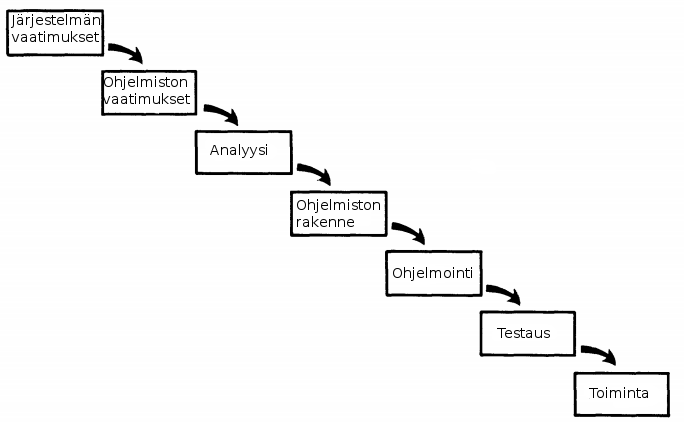
\includegraphics[width=\textwidth]{waterfall}
\end{figure}

Kuvassa 1. on kuvaus lineaarisesta vesiputousmallista. Winston Royce jaotteli vesiputousmallissa ohjelmistotuotannon vaiheet seuraavasti: järjestelmän ja ohjelmiston vaatimusmäärittely sekä analyysi, ohjelmistonrakenteen suunnittelu, ohjelmointi, testaus ja ohjelmiston käyttö \cite{ROY70}.

Määrittely- ja analyysivaiheessa kerätään kehitettävän järjestelmän ja ohjelmiston vaatimukset ja rajoitteet. Vaatimukset ovat joukko toiminnallisuuksia, joita loppukäyttäjä odottaa ohjelmistolta. Loppukäyttäjien vaatimuksien ja liiketoimintaympäristön analysointi on edellytys ohjelmiston rakenteen suunnittelulle. \cite{ROY70}.

Seuraavassa vaiheessa suunnitellaan järjestelmän rakenne: ohjelmiston arkkitehtuuri, tarvittavat luokat ja niiden toiminnallisuus sekä komponenttien yhteensopivuus ja yhteistoiminta. \cite{ROY70}.

Ohjelmointivaiheessa kirjoitetaan ohjelmakoodi laadittujen suunnitelmien perusteella. Testausvaiheessa varmistetaan, että rakennettu ohjelmistojärjestelmä toimii vaatimusten mukaan. Toimintavaiheessa ohjelmisto on loppukäyttäjillä operatiivisessa toiminnassa \cite{ROY70}. 

Artikkelissaan Royce kirjoittaa, että testauksen tulisi tehdä siihen erikoistuneet henkilöt, jotka eivät välttämättä ohjelmoineet itse alkuperäistä ohjelmiston osaa. Useimmat virheet ovat luonteeltaan ilmiselviä, jotka voidaan löytää visuaalisella tarkastelulla. Jokaisen analyysin ja ohjelmakoodin tulee tarkastaa toinen henkilö, joka ei osallistunut varsinaiseen työhön. Jokainen tietokoneohjelman looginen polku on testattava ainakin kerran \cite{ROY70}.

Royce painottaa dokumentin tärkeyttä, jotta testaaja voisi ymmärtää ohjelmiston toimintaa. Hyvän dokumentoinnin todellinen arvo ilmenee testausvaiheessa, ohjelmistoa käytettäessä sekä uudelleen suunniteltaessa. Hyvän dokumentin avulla esimies voi keskittää henkilöstön ohjelmistossa ilmenneisiin virheisiin. Ilman hyvää dokumenttia, ainoastaan ohjelmistovirheen alkuperäinen tekijä kykenee analysoimaan kyseessä olevan virheen. Käyttöönotossa ilmenneiden ohjelmistovirheiden korjaamisessa selkeä dokumentti on välttämätön \cite{ROY70}.

Dokumentaatio on tärkeä osa suunnitelmavetoisia ohjelmistotuotantomenetelmiä. Dokumentin tulee olla ymmärrettävä, valaiseva ja ajantasainen dokumentti, ja jokaisen työntekijän on sisäistettävä se. Vähintään yhden työntekijällä on oltava syvällinen ymmärrys koko järjestelmästä, mikä on osaltaan saavutettavissa dokumentin laadinnalla. Ohjelmistosuunnittelijoiden on kommunikoitava rajapintojen (interface) suunnittelijoiden ja projektin johdon kanssa. Dokumentti antaa ymmärrettävän perustan rajapintojen suunnitteluun ja hallinnollisiin ratkaisuihin. Kirjallinen kuvaus pakottaa ohjelmistosuunnittelijan yksiselitteiseen ratkaisuun ja tarjoaa konkreettisen todistuksen työn valmistumisesta. Dokumentti helpottaa ohjelmiston käyttöönottoa operatiivinen henkilöstön kanssa.  	  

\subsection{Spiraalimalli}

Barry Boehm esitteli artikkelissaan ''A Spiral Model of Software Development and Enhancement'' spiraalimallin (spiral model). Mallin tarkoitus oli edistää ohjelmistotuotantoprosessia lähestymällä ohjelmistoa riskivetoisesti. Tämä mahdollistaa mallin mukautumaan, kohdattavien riskien mukaan, sopivasti yhdistelemällä määrittelyä (specification), prototyyppien valmistusta, simulointia tai muita lähestymistapoja ohjelmiston suunnitteluun \cite{BOE88}.


Kuvassa 2. on spriraalimalli, joka on kehitetty vesiputousmallista saatujen useiden vuosien kokemuksien perusteella. Malli kuvastaa taustalla olevaa käsitettä, että jokainen vaihe sisältää saman sarjan toimenpiteitä \cite{BOE88}.

\begin{figure}[h!]
  \caption{Spiraalimallin ohjelmiston elinkaari}
  \centering
    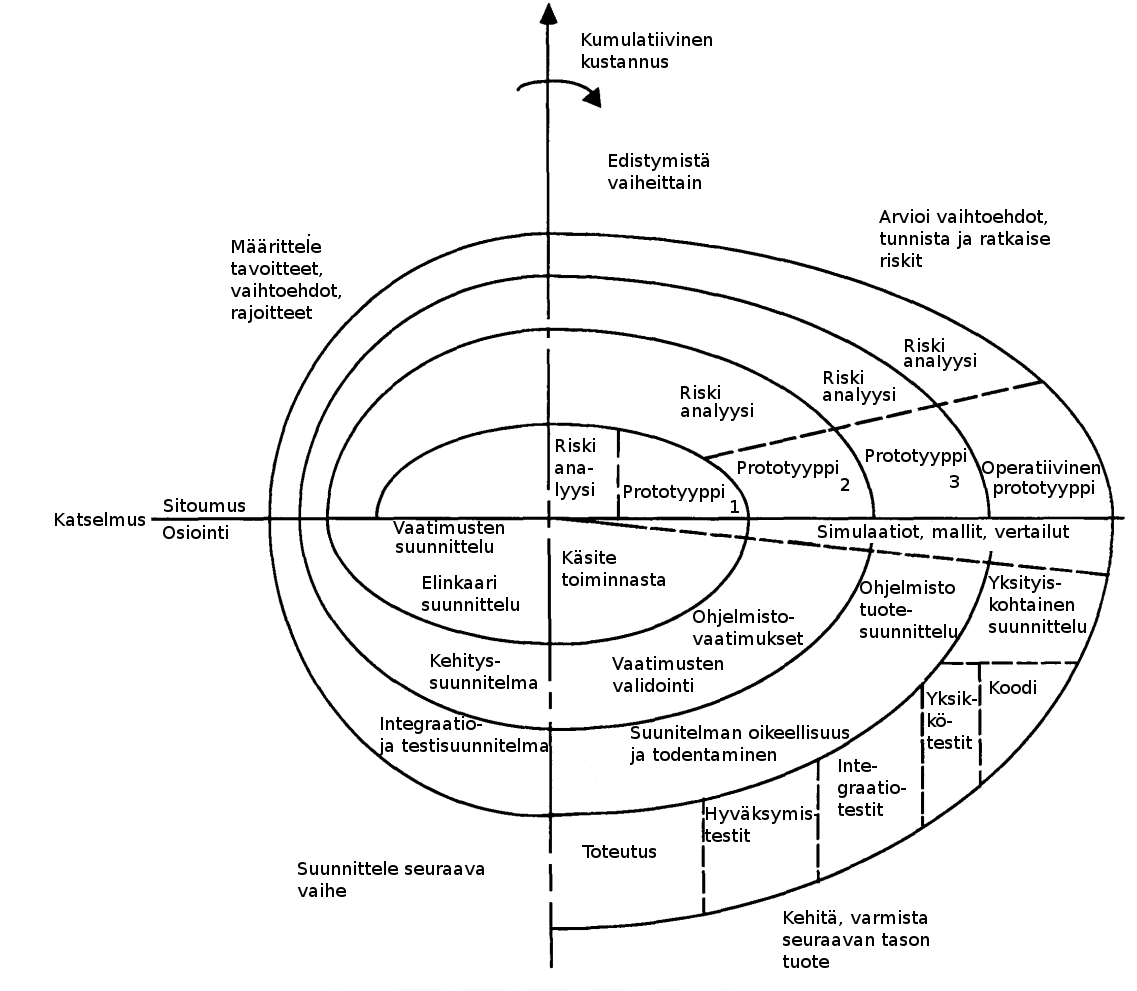
\includegraphics[width=\textwidth]{spiral}
\end{figure}

Spiraalimallissa jokainen vaihe aloitetaan tunnistamalla:
\begin{itemize}
  \item laadittavien ohjelmisto-osien suorituskykyyn, toiminnallisuuteen sekä sopeutumiskykyyn liittyvät tavoitteet
  \item vaihtoehtoiset toteutustavat (ohjelmiston osto, ohjelmiston uudelleenkäyttö, vaihtoehtoiset ohjelmat)
  \item ohjelmiston eri vaihtoehdoille asettamien rajoitteet (rajapinnat, aikataulu, kustannukset) \cite{BOE88}.
\end{itemize}

Seuraava askel on arvioida vaihtoehtoja suhteessa ohjelmiston tavoitteisiin ja rajoitteisiin. Usein tämä prosessi tunnistaa epävarmoja alueita, jotka ovat merkittäviä riskin lähteitä. Riskien löytyessä, seuraava askel pitää sisällään kustannustehokkaan strategian muotoilun riskien ratkaisemiseksi. Tähän voi liittyä prototyyppien valmistamista, simulointia, vertailuanalyysia, kyselylomakkeita, analyyttista mallinnusta, tai näiden yhdistelmiä sekä muita riskien ratkaisumenetelmiä \cite{BOE88}.

Jos suorituskykyyn tai käyttöliittymään liittyvät riskit hallitsevat ohjelman kehittämistä, seuraavassa vaiheessa määritellään ohjelmiston yleistä luonnetta, suunnitellaan seuraavan tason prototyyppiä ja kehitetään yksityiskohtaisempaa prototyyppiä riskien ratkaisemiseksi \cite{BOE88}.

Riskinhallinta huomioiden voidaan määritellä kiinnitettävä aika ja työmäärä toiminnan suunnitteluun (planning), asetuksien hallintaan (configuration management), laadun varmistukseen (quality assurance), muodolliseen todentamiseen (formal verification) ja testaukseen \cite{BOE88}.

Spiraalimallin tärkeä ominaisuus on, että jokainen iteraatio päätetään katselmukseen tuotteeseen liittyvän henkilöstön tai organisaation kanssa \cite{BOE88}.

Spriraalimallissa yksikkö-, integraatio- ja hyväksymis\-testit ovat ohjelmiston kehityskaaren lopussa \cite{BOE88}. Spriraalimallin riskiperustaisesta lähestymistavasta huolimatta, ohjelmiston kehitysprosessi sisältää riskejä ohjelmiston laatuun ja testaukseen liittyen. 

\section{Ketterät kehitysmenetelmät}

Ketterät menetelmät (agile methods) ovat saavuttaneet suosiota ohjelmistotuotannossa. Usein iteraatiivisia, inkrementaalisia sekä kehityksellisiä (evolutionary) menetelmiä pidetään modernina ohjelmistokehityksenä, mikä on korvannut vesiputousmallin. Mutta näitä menetelmiä on käytetty vuosikymmeniä \cite{LAB03}.

Monet ohjelmistotuotantoprojektit  (esimerkiksi NASA:n Mercury- ja avaruussukkula-projektit) 1970- ja 1980-luvulla käyttivät iteraatiivisia ja inkrementaalisia menetelmiä.  Menetelmillä oli eroavaisuuksia iteraatioiden pituuksissa ja aikarajoitteiden käytössä (time-box). Joillakin oli merkittävä suunnittelu- ja vaatimusmäärittelyvaihe (big design up front), jota seurasi inkrementaalinen aikarajoitettu (time-box) kehitysvaihe. Toisilla oli enemmän kehityksellisempi ja palautteen ohjaama lähestymistapa \cite{LAB03}.

Eroavaisuuksista huolimatta, kaikilla lähestymistavoilla oli yhteistä välttää, lineaarista vaihe kerrallaan etenevää, suunnitelma- ja dokumenttivetoista menetelmää \cite{LAB03}.

Suunnitelmavetoisten prosessimallien ongelmien seurauksena useat ohjelmistoalan ihmiset ja organisaatiot kehittivät menetelmiä ja käytäntöjä, joille muutokset ovat hyväksyttyjä. Nämä uudet menetelmät toivottavat muutokset tervetulleiksi, ja ohjelmisto kehittyy uusiin vaatimuksiin ja muutoksiin mukautuen \cite{WIC03}. Perinteinen lähestymistapa perustui oletukselle, että aikaisella ja täydellisellä vaatimusmäärittelyllä voidaan pienentää kustannuksia vähentämällä muutoksia. Nykyään muutosten kieltäminen merkitsee reagoimattomuutta liiketoimintaympäristön kehitykselle \cite{HIC01}.

Menetelmiä kehitettiin useita ja eri maissa: 
\begin{itemize}
 \item taipuisa järjestelmän kehitysmenetelmä (Dynamic Systems Development) Euroopassa
 \item toiminnallisuusvetoinen kehitysmenetelmä (Feature-Driven Development) Australiassa
 \item ja XP (Extreme Programming) \cite{BEC99}, Crystal \cite{COC05}, mukautuva ohjelmistokehitys (Adaptive Software Development) ja Scrum \cite{SCH09} Yhdysvalloissa \cite{WIC03}.
\end{itemize}

Helmikuussa 2001 17 menetelmien kehittäjää tapasi keskustellakseen kevyistä menetelmistä ja kokemuksiensa yhtäläisyyksistä. Huomatessaan, että heidän käytänteillään oli paljon yhteistä, ja että heidän prosessinsa tarjosivat keinoja saavuttaa merkityksellinen päämäärä: asiakkaan tyytyväisyys ja korkea laatu \cite{WIC03}. 

Osallistujat määrittelivät käytännöt ketteriksi menetelmiksi.
Osallistujat kirjoittivat ''Manifesto for Agile Software Development''-julistuksen, mikä kuvaa ketterän kehityksen perusarvoja:

\begin{itemize}
 \item yksilöt ja vuorovaikutus ennen prosesseja ja työkaluja
 \item toimiva ohjelmisto ennen kattavaa dokumentaatiota
 \item asiakasyhteistyö ennen sopimusneuvotteluja
 \item muutoksiin vastaaminen ennen suunnitelman seuraamista \cite{WIC03}.
\end{itemize}

Ohjelmistotuotannon parissa työskentelevät huomasivat, että ohjelmistoinsinööritieteet erosivat huomattavasti muista insinööritieteistä. Autojen kokoaminen on määriteltävä prosessi. Insinöörit voivat suunnitella prosessin, määritellä kokoonpanojärjestyksen sekä työntekijöiden, koneiden tai robottien toimenpiteet \cite{WIC03}.

Ohjelmistotuotantoprojektit ovat luonteeltaan empiirisiä prosesseja, joiden lopputuloksena syntyy uusia tuotteita. Projektin aikana on oleellista oppia ja mukautua prosessin edetessä, eikä määritellä kaikkea alussa kattavasti. Empiirinen prosessi vaatii \textit{tarkkaile ja mukaudu} (\textit{inspect and adapt}) tyyppisen lähestymistavan. Lyhyet iteraatiot auttavat ketteriä menetelmiä mukautumaan ja muuttamaan ohjelmistoteollisuuden ennustamattomien vaatimuksien mukaan \cite{WIC03}.

\subsection{Extreme programming}

XP (Extreme Programming) vähentää ohjelmiston vaatimusten muuttumisen kustannuksia tekemällä koko kehityskaaren aikaisia toimintoja jatkuvasti ohjelmistokehityksen aikana. Perinteisen ohjelmistotuotantoprosessin sijaan suunnitellaan, analysoidaan ja muotoillaan rakennetta jokaisessa iteraatiossa \cite{BEC99}.

Jatkuvasti paikalla oleva asiakas (on-site customer) valitsee mahdollisimman pienen määrän toiminnallisuuksia, jotka tuottavat eniten arvoa ohjelmistolle ja toimivat julkaistavana ohjelmistona (release). Määrätyt toiminnallisuudet toteutetaan ensin ja ohjelmisto julkaistaan. Asiakkaan on priorisoitava tärkeimmät toiminnallisuudet, jotka hän haluaa ohjelmistoon toteutettavan ensimmäisenä \cite{BEC99}.

Suunnitteluprosessin (planning game) aikana tiimi määrittää toiminnallisuuksille hinnan - aika-arvion. Arvio saadaan jakamalla tiimin tekemät toiminnallisuudet toteutukseen vaaditulla aikayksiköllä. Julkaisun budjetti lasketaan toivottujen toiminnallisuuksien aika-arvioiden perusteella. Asiakas voi valita halutut toiminnallisuudet ja pyytää tiimiä laskemaan julkaisupäivän. Tai asiakas voi valita julkaisupäivän ja valita tarinoita julkaisuun kunnes budjetti täyttyy \cite{BEC99}.

Ohjelmisto laitetaan tuotantoon nopealla aikataululla. Uusia versioita julkaistaan usein - kuukausittain tai jopa päivittäin. Uutta ohjelmakoodia integroidaan nykyiseen ohjelmistoon jopa muutaman tunnin välein (continuos integration). Integroidessa uutta koodia koko järjestelmä rakennetaan alusta uudestaan ja kaikki testit ovat läpäistävä, tai kaikki muutokset hylätään \cite{BEC99}.

Asiakas valitsee seuraavaan iteraatioon eniten arvoa tuottavat tarinat (story), jotka ovat arviotavissa ja testattavissa. Ohjelmoijat jakavat tarinat pieniksi tehtäviksi (task). Ohjelmoijat muuttavat tehtävät joukoksi testejä, jotka osoittavat tehtävän valmistuneen. Parin kanssa työskentelemällä ohjelmoija ajaa testejä ja kehittää samalla mahdollisimman yksinkertaista suunnitelmaa tehtävän ratkaisemiseksi \cite{BEC99}.  

Jokaisen iteraation tarkoituksena on lisätä ohjelmistoon uusia toiminnallisuuksia, jotka ovat testattuja ja valmiita. Prosessi alussa asiakas ja ohjelmoijat suunnittelevat joukon tarinoita, jotka toteutetaan ohjelmistoon. Iteraatiota suunniteltaessa asiakas valitsee eniten arvoa tuottavat toiminnallisuudet. Tiimi pilkkoo toiminnallisuudet pienemmiksi tehtäviksi. Tehtävät ovat toiminnallisuuden osia, jotka yksi ohjelmoija voi toteuttaa muutamassa päivässä. Asiakas laatii hyväksymistestit tarinalle (functional test) ja tiimi toteuttaa vaaditun toiminnallisuuden. Iteraation lopussa testit ajetaan hyväksytysti ja prosessi on valmis seuraavaan iteraatioon \cite{BEC99}.

Toteuttaakseen tehtävän (task) ohjelmoijat työskentelevät pareittain, jos ilmenee kysymyksiä toteutuksesta tai toiminnallisuuden laajuudesta pari keskustelee hetken jatkuvasti paikalla olevan asiakkaan (on-site customer) kanssa. Pari tiivistää toiminnallisuuden testitapauksiksi, jotka ovat ajettavissa ennen kuin tehtävä on valmis. Testit luovat pohjan tuotettavalle ohjelmakoodille ja pari pyrkii mahdollisimman yksinkertaiseen tapaan ratkaista testitapaukset. Kun ohjelmakoodi läpäisee testit, ohjelmoijat suunnittelevat rakennetta uudelleen (refactoring), jos on tarvetta \cite{BEC99}.     

XP:ssä testausta painotetaan paljon. Kaikki ohjelmoijat testaavat tehdessään tuotantokoodia. Ohjelmoijat liittävät uudet testitapaukset ja tuotetut toiminnallisuudet ohjelmistoon. Tämä varmistaa jatkuvan integraation (continuos integration) ja vaakaan rakennusprosessin \cite{FOW01a}.

Ohjelmoijat kirjoittavat testin toiminnallisuudelle ennen tuotantokoodia. Testit ovat jatkuvasti osana ohjelmistoa. Iteraation alussa asiakas päättää miten vakuuttaa, että uusi tarina on lisätty onnistuneesti ohjelmistoon. Hänen päätökset, uuden toiminnallisuuden toimivuudesta, muutetaan koko järjestelmän laajuisiksi testeiksi. Testit takaavat ohjelmoijille ja sidosryhmille, että ohjelmisto toimii ja täyttää odotetut vaatimukset. Testit ovat ajettavissa koko ohjelmiston kehityskaaren ajan, mikä takaa ohjelmiston toimivuuden, kun lisätään uusia toiminnallisuuksia tai ohjelmakoodin rakennetta muutetaan \cite{BEC99}.

Winston Royce kirjoitti artikkelissaan ''Managing the development of large software systems'', että ohjelmoijan ei tule testata kirjoittamaansa ohjelmakoodia. Royce arvioi, että useimmat virheet ovat ilmiselviä ja ovat löydettävissä katsomalla ohjelmakoodia \cite{ROY70}. XP:ssä tätä ongelmaa on lähestytty työskentelemällä jatkuvasti pareittain \cite{BEC99}. 


\subsection{Scrum}

Scrum lähestyy ohjelmistotuotantoprojektin monimutkaisuutta joukolla yksinkertaisia käytänteitä ja sääntöjä. Scrum on tarkasteleva, mukautuva ja empiirinen prosessi. Scrum perustaa kaiken käytännön iteratiiviselle ja inkrementaaliselle prosessille. Jokaisen iteraation tulos on ohjelmistotuotteen inkrementaalinen edistyminen. Iteraatioita vie eteenpäin lista vaatimuksista \cite{SCH09}. 

Iteraation alussa tiimi selvittää mitä sen on tehtävä. Tiimi harkitsee saatavilla olevia teknologioita, arvio omia taitojaan ja kykyjään. Tiimi yhdessä päättää miten uusi toiminnallisuus toteutetaan, mukautuen vaikeuksiin ja yllätyksiin. Tiimi työskentelee rauhassa parhaan kykynsä mukaan lopun iteraation ajan. Iteraation lopussa tiimi esittelee toiminnallisuuden sidosryhmille, jotka tarkastelevat toiminnallisuutta ja tarvittavat muutokset voidaan tehdä riittävän ajoissa \cite{SCH09}.

Scrum määrittää kolme eri roolia: tuoteomistaja (Product owner), kehittäjätiimi (Team) ja scrummaster (Scrum master). Kaikki projektin hallinnolliset vastuut on jaettu näiden roolien kesken. Tuoteomistajan vastuu on esitellä sidosryhmän, projektin lopulliselle tuotteelle asetettavat, vaatimukset. Tuoteomistaja laatii alustavan vaatimusmäärittelyn, sijoitettavalle pääomalle asetettavat tavoitteet (ROI) ja julkaisu suunnitelmat (relese plans). Tuoteomistaja vastaa, että vaatimuslistan (Product backlog) eniten arvoa tuottavat toiminnallisuudet toteutetaan ensin. Tuoteomistaja priorisoi vaatimuslistan toiminnallisuuksia. Näin seuraavassa iteraatiossa lisätään eniten arvoa tuottavat toiminnallisuudet ensin \cite{SCH09}. 

Tiimin vastuulla on toiminnallisuuksien kehittäminen. Tiimi on monipuolisesti eri alojen asiantuntemuksen omaamista ihmisistä koostuva ryhmä ja se on itse-organisoituva. Heidän tehtävä on vaatimuslistan toiminnallisuuksien lisääminen inkrementaalisesti iteraation aikana. Tiimi on yhdessä vastuussa jokaisen iteraation onnistumisesta. Scrummaster on vastuussa itse Scrum prosessista. Hänen tehtävänä on esitellä Scrumin periaatteet jokaiselle projektiin osallistuvalle, sekä toteuttaa Scrumia niin, että se sopii organisaation kulttuuriin ja toteuttaa odotetut hyödyt. Scrummaster valvoo, että jokainen toteuttaa ja seuraa Scrumin periaatteita \cite{SCH09}.

Tuoteomistajalla on olemassa tuotettavasta ohjelmistosta näkemys. Tuoteomistajan visio konkretisoituu listana vaatimuksista tuotteen kehitysjonona (product backlog). tuotteen kehitysjono on priorisoitu: toiminnallisuudet jotka tuottavat arvoa ovat ylimpänä listassa. Tuotteen kehitysjono on projektin lähtökohta ja sen sisältö, prioriteetit ja ryhmittely julkaisuihin yleensä muuttuvat projektin käynnistyttyä. Muutokset tuotteen kehitysjonossa heijastavat muuttuvaa liiketoimintaympäristöä ja tiiimin nopeutta toteuttaa toiminnallisuuksia \cite{SCH09}.

Sprintin tehtävälista (Sprint backlog) sisältää tiimin määrittelevät tehtävät, joita tiimi toteuttaa. Tehtävät ovat tuotteen kehitysjonosta sprinttiin valittuja toiminnallisuuksia, jotka tiimi on pilkkonut pienempiin osiin. Jokainen tehtävä tulisi olla noin 4-16 tunnin pituinen ohjelmointitehtävä. Ainoastaan tiimi voi muuttaa sprintin tehtävälistaa. Sprintin tehtävälista on läpinäkyvä, reaaliaikainen kuva, mitä tiimi pyrkii saavuttamaan kyseessä olevassa sprintissä. Tehtävän yhteydessä on kirjattu arvio ajasta, jonka kyseessä olevaan tehtävään on arvioitu kuluvan, ja henkilö kuka on vastuussa kyseisestä tehtävästä \cite{SCH09}.

Kaikki työ tehdään 30 päivän iteraatioissa (Sprint). Jokainen sprintti alkaa iteraation suunnittelupalaverilla (Sprint planning meeting), jossa tuoteomistaja ja tiimi yhteistyössä päättävät mitä toteutetaan. Valitsemalla tuotteen kehitysjonosta korkeimman prioriteetin toiminnallisuudet tuoteomistaja kertoo mitä hän toivoo ja tiimi selvittää miten paljon toivomuksista he voivat muuttaa toiminnallisuuksiksi seuraavassa sprintissä \cite{SCH09}.

Joka päivä tiimi kokoontuu 15 minuutin tapaamiseen - päiväpalaveriin (Daily Scrum). Jokainen tiimin jäsen vastaa kolmeen kysymykseen: Mitä olen tehnyt viimeisen tapaamisen jälkeen? Mitä ajattelin tehdä seuraavaksi? Mikä estää minua saavuttamasta tavoitteitani? Tapaamisen tarkoituksena on synkronoida tiimin työ päivittäin ja sopia tapaamisista, joita tiimi tarvitsee edetäkseen työssään \cite{SCH09}.

Iteraation lopussa pidetään sprinttikatselmus (Sprint review meeting), jossa tiimi esittelee tuoteomistajalle ja muille sidosryhmille, jotka haluavat osallistua, mitä tiimi on kehittänyt iteraation aikana. Tapaamisen tarkoituksena on tuoda ihmiset yhteen, esitellä ohjelmiston toiminnallisuudet ja auttaa osallistujia yhdessä päättämään, mitä tiimin tulisi seuraavaksi tehdä \cite{SCH09}. 

Sprinttikatselmuksen jälkeen ja ennen seuraavan sprintin suunnittelupalaveria, scrummaster ja tiimi pitää sprintin retrospektiivin (Sprint retrospective meeting). Scrummaster rohkaisee tiimiä kertaamaan kehitysprosessiaan, tehdäkseen siitä tehokkaampaa ja nautittavampaa seuraavaan iteraatioon \cite{SCH09}.

Yhdessä sprintin suunnittelupalaveri, päiväpalaveri, sprinttikatselmus ja sprintin retrospektiivi muodostavat scrumista empiirisen, tarkastelevan ja sopeutuvan projektinhallintakehyksen \cite{SCH09}.

Scrumissa on kaikkien tiimin jäsenten oltava selvillä määritelmästä ''valmis toiminnallisuus''. Scrum vaatii tuotteeseen lisättävän toiminnallisuuden olevan kattavasti testattu, rakenteeltaan hyvin suunniteltua ja kirjoitettua ohjelmakoodia, ja toiminnallisuus on oltava dokumentoituna operaation käyttäjälle. Tuotteella saattaa olla lisäksi muita vaatimuksia standardien tai käytänteiden muodossa \cite{SCH09}.

\section{Ohjelmiston laatu}

Ohjelmistokehittäjien on otettava laatu huomioon sekä suurissa monimutkaisissa ohjelmistojärjestelmissä että pienissä sulautetuissa ohjelmistoissa. Ohjelmistossa ilmeneviä virheitä sallitaan enemmän tekstinkäsittelyohjelmassa kuin ydinvoimalalaitoksen ohjausjärjestelmissä \cite{KIP96}. Oletetaan, että tilattu ohjelmistojärjestelmä toimitetaan ajallaan ilman budjettia ylittäviä kustannuksia, ja se toimii oikein sekä suorittaa tehokkaasti sille määritetyt toiminnallisuudet. Voidaanko tuotteeseen tällöin olla tyytyväisiä? Ei välttämättä kaikissa tapauksissa \cite{BBL76}.

Ohjelmistojärjestelmää voi olla vaikea ymmärtää ja muuttaa. Ohjelmistoa ei välttämättä ole helppokäyttöinen. Ohjelmisto voi olla tarpeettoman laitteistoriippuvainen. Nämä seikat johtavat kohtuuttomiin ylläpitokustannuksiin \cite{BBL76}.       

Kansainvälinen standardointi organisaatio (ISO) on suositellut laadun perustaksi kuusi itsenäistä piirrettä:

\begin{enumerate}
  \item toiminnallisuus (functionality)
  \item luotettavuus (reliability)
  \item käytettävyys (usability)
  \item tehokkuus (efficiency)
  \item ylläpidettävyys (maintainability)
  \item siirrettävyys (portabilty) \cite{KIP96}
\end{enumerate}

Ohjelmiston toiminnallisuuksien on tyydytettävä todetut ja epäsuorat vaatimukset sekä kyettävä ylläpitämään ilmoitettu suoritustaso vaadituissa tilanteissa siltä vaaditun ajan. Käytettävyyden on vastattava oletettua ohjelmiston käytöstä aiheutuvaa vaivannäköä. Tehokkuus ilmaisee suorituskyvyn ja käytettyjen resurssien suhdetta todetuissa olosuhteissa. Ylläpidettävyys ilmaisee vaaditun vaivannäön määriteltyihin muutoksiin, jotka voivat liittyä korjauksiin, parannuksiin tai ohjelmiston mukauttamista muuttuneisiin olosuhteisiin. Siirrettävyys viittaa ohjelmiston kykyyn toimia erilaisessa ympäristössä: toisessa organisaatiossa, laitteistossa tai ohjelmistoympäristössä \cite{KIP96}.

\subsection{Ohjelmiston suunnittelu}

Suunnitelmavetoisissa menetelmissä ohjelmistosuunnittelijat suunnittelevat etukäteen isoa kokonaiskuvaa koko järjestelmästä. Suunnittelijoiden ei tarvitse miettiä jokaista pientä yksityiskohtaa, koska suunnittelutekniikat, kuten UML (unified modeling language) antavat mahdollisuuden työskennellä abstraktimmalla tasolla. Suunnittelijoiden ei tarvitse ottaa huomioon käytännön ohjelmointia ja sen aiheuttamaa entropiaa. Suunnittelijan on kuitenkin mahdotonta ottaa huomioon kaikkia yksityiskohtia, mitä ohjelmoija joutuu ratkaisemaan yksityiskohtaisemmalla tasolla \cite{FOW01b}.

\textit{ohjelmoi ja korjaa}-menetelmä, jossa suunnitelma on ainoastaan perättäisiä erillisiä taktisia päätöksiä, johtaa tavallisesti vaikeasti muutettavaan ohjelmakoodiin. Voidaan sanoa ettei tällainen ole suunniteltua ohjelmistokehitystä. Tai ainakin tällainen menettely johtaa huonoon ohjelmiston rakenteeseen. Suunnitelman heikentyessä vaikeutuu kyky tehdä muutoksia tehokkaasti \cite{FOW01b}. 

Ohjelmistoprojektin edetessä ja entropian lisääntyessä ohjelmiston rakenne huononee. Tämä ei ainoastaan vaikeuta ohjelmiston muuttamista, vaan lisää virheiden määrää. Ja virheiden löytäminen sekä niiden poistaminen ohjelmistosta vaikeutuu. Tällainen on \textit{ohjelmoi ja korjaa}-menetelmän tyypillinen ongelma: ohjelmistovirheiden korjaaminen on eksponentiaalisesti kalliimpaa projektin edetessä \cite{FOW01b}.

Winston Roycen vesiputousmalli \cite{ROY70} ja Barry Boehmin spriraalimalli \cite{BOE88} perustavat ohjelmistokehityksen vahvasti dokumentti- ja suunnitelmavetoisille prosessille, jossa tuotettavaa ohjelmistoa ja ongelma-aluetta pyritään lähestymään analyysin, vaatimusmäärittelyn sekä suunnittelun kautta. Molemmissa malleissa ratkaisuksi ohjelmistotuotannon ongelmiin esitetään prototyypin valmistamista, mitä testaamalla ilmeneviin ongelmiin voidaan reagoida mahdollisimman aikaisin.

Royce ehdottaa vesiputousmallissa, että prototyypin kehityksen aikataulu on kolmannes varsinaisen tuotteen kehitykseen vaaditusta ajasta \cite{ROY70}. Boehm ei määritellyt spiraalimallissa iteraatioiden pituutta suhteessa ohjelmistokehitykseen vaadittuun aikaan. Mutta spiraalimallissa Boehm painottaa vahvasti prototyypin osuutta ohjelmiston kehityskaaren aikana. Varhainen prototyyppi tarjoaa ohjelmiston testattavaksi, jotta virheitä voidaan löytää aikaisessa vaiheessa. Asiakkaan kanssa tehdyssä katselmuksessa saadaan prototyypistä palautetta seuraavan iteraation prototyyppiin \cite{BOE88}.

Erityisesti Royce painotti artikkelissaan ''Managing the development of large software systems'' dokumentoinnin tärkeyttä \cite{ROY70}. Suunnitelmavetoisten prosessien mukautuminen muuttuviin muutoksiin vaikeutuu kattavan dokumentoinnin takia. Nopeasti muuttuvat vaatimukset tekevät dokumenteista vanhentuneita, ja niiden päivittäminen vaati aikaa. Turhien kaavioiden piirtämiseen kuluu kalliita resursseja, kun suunnitelmat muuttuvat. Kaaviot vanhentuvat ja käyvät tarpeettomiksi \cite{FOW01b}.

Edellä kuvatuissa ketterissä ohjelmistotuotannon menetelmissä on yhteistä pyrkimys formaalilla tavalla määritellä ohjelmistotuotannon prosessi, jolla voidaan välttää ''ohjelmoi ja korjaa''-menetelmän ja suunnitelmavetoisten prosessien ongelmat. Suunnitelmavetoisissa menetelmissä on pyritty tehostamaan vaatimusmäärittelyprosessia, jotta vaatimukset voidaan kattavasti määritellä ja välttää muutoksia ohjelmistokehityksen edetessä. Monia odottamattomia muutoksia vaatimuksissa tapahtuu kuitenkin koska liiketoimintaympäristö muuttuu \cite{FOW01b}.

Ketterien menetelmien prosesseissa suunnittelussa painotetaan joustavuutta, jotta suunnitelmaa voidaan helposti muuttaa kun vaatimukset muuttuvat. XP:ssä suunnitelmien ja kaavioiden merkitys on vähäinen: UML kaavioita tulisi käyttää, jos niistä on hyötyä. Äärimäiset XP:n toteuttajat eivät käytä UML-kaavioita lainkaan \cite{FOW01b}. Kaavioiden merkitys on tarjota yhteydenpitoa. Tehokkaan yhteydenpidon takaamiseksi on piirrettävään kaavioon valittava tärkeät asiat ja vältettävä vähemmän tärkeitä. Vain merkitykselliset luokat sekä niiden tärkeimmät attribuutit ja operaatiot tulee kuvata UML-kaavioon \cite{FOW01b}.

Tehtyä kaaviota on pidettävä luonnoksena ei valmiina suunnitelmana. Ohjelmoinnin edetessä usein selviää, että jotkin suunnitelman osa-alueet ovat vääriä. Usein ongelma ei ole suunnitelmien muuttamisessa. Ongelmana on, että usein ihmiset ajattelevat suunnitelman olevan valmis, eivätkä vie ohjelmoidessa saatua tietoa takaisin suunnitelmaan \cite{FOW01b}. 

Suunnitelmien muututtua ei kaaviota tarvitse välttämättä muuttaa. On täysin perusteltua piirtää kaaviota ymmärtääkseen ohjelmiston rakennetta ja heittää kaaviot toteutuksen jälkeen pois. Kaavioiden piirtämisen hyöty on jo saavutettu rakenteen suunnittelulla ja sen ymmärtämisellä. Kaavioiden ei tule olla pysyviä suunnitelman osia \cite{FOW01b}.

Ohjelmoinnin aikaista dokumentointia voidaan muuttuviin vaatimuksiin ja suunnitelmiin sopeuttaa seuraavasti:

\begin{itemize}
 \item Käytetään vain kaavioita, joita voidaan pitää ajan tasalla helposti 
 \item Laitetaan kaaviot paikkaan, jossa ne ovat helposti nähtävillä
 \item Kannustetaan ihmisiä muuttamaan kaavioita
 \item Heitetään pois kaaviot joita ihmiset eivät käytä \cite{FOW01b}.
\end{itemize}

Usein UML-kaavioita käytetään välittämään tietoa eri ryhmien välillä. XP:n näkökulmasta UML-kaaviot ovat tarinoita muiden joukossa, joiden arvon määrää asiakas. UML-kaaviot ovat hyödyllisiä vain jos ne auttavat viestinnässä. Ohjelmakoodin varasto (repository) on yksityiskohtaisen tiedon lähde ja kaaviot koostavat ja korostavat tärkeitä asioita \cite{FOW01b}.    


\subsection{Ohjelmiston testaus}


\subsection{Pariohjelmointi}

Pariohjelmoinnissa kaksi ohjelmoijaa yhdessä työstävät yhtä ohjelmakoodia, algoritmia tai suunnitelmaa. Toinen parista, ajaja, ohjelmoi ja toinen aktiivisesti tarkkailee ajajan työtä, etsien virheitä, miettien vaihtoehtoja, tutkien lähteitä ja miettien strategisia toteutustapoja. Parit vaihtavat roolejaan jaksoittain. Molemmat ovat tasavertaisia ja aktiivisia osallistujia \cite{WIL00}.

Pariohjelmoinnin kustannukset ovat oleellinen asia. Jos kustannukset ovat suuret, johtajat eivät salli pariohjelmointia. Epäluuloiset olettavat, että pariohjelmoinnin sisällyttäminen ohjelmistotuotantoon kaksinkertaistaa kustannukset jos henkilöstömäärää on lisättävä samassa suhteessa. Tutkimukset kuitenkin osoittavat, että pareittain työskentelevät tiimit suoriutuvat tehokkaammin kuin yksittäiset ohjelmoijat \cite{NOS98} \cite{WIL00}.

Pareittain työskentelevät tuottavat luettavampaa ohjelmakoodia ja toimivampia ratkaisuja kuin yksin toimivat ohjelmoijat. Ryhmissä toimivat ratkaisevat ongelmia keskimäärin nopeammin kuin yksilöt. Lisäksi pareittain toimivat ilmaisevat korkeampaa luottamusta ratkaisuunsa ja kokevat nauttivansa prosessista enemmän kuin yksin toimivat ohjelmoijat \cite{NOS98}.   

Pariohjelmointi tuottaa erityisesti parempaa suunnittelua ja analyysia kuin yksilölliset ohjelmoijat. Pari harkitsee huomattavasti enemmän vaihtoehtoja ja yhtyvät nopeasti toteutettavaan ratkaisuun. Ideoiden vaihto parin välillä merkittävästi vähentää huonon rakennesuunnitelman todennäköisyyttä.  Yhdessä työskentelemällä pari voi toteuttaa tehtäviä, jotka voivat olla liian haastavia yhdelle. Parityöskentely pakottaa osallistujia keskittymään täysin haasteena olevaan tehtävään \cite{WIL00}.

Vuonna 1998 John Nosek teki tutkimuksen, jossa kokeneet ohjelmoijat työskentelivät haastavien, omalle organisaatiolleen tärkeiden, tehtävien parissa omassa työskentely-ympäristössään. Kukaan osallistujista ei ollut työskennellyt annetun tehtävän kaltaisen ongelman parissa aikaisemmin. Annetun tehtävän kaltaista ongelmaa pidettiin organisaatiolle menestykselle tärkeänä ja niin vaativana, että yleensä tehtäviin palkattiin ulkopuolisia konsultteja \cite{NOS98}.

Koehenkilöt valittiin satunnaisesti työskentelemään pareittain testiryhmään ja yksilöinä kontrolliryhmään.
Ryhmiltä tehtäviin kulunut aika mitattiin. Ratkaisuista pisteytettiin luettavuus väliltä 0-2. Lukuarvo 0 tarkoitti lukukelvotonta ratkaisua ja 2 täysin luettavissa olevaa ratkaisua. Ratkaisun toimivuus pisteytettiin väliltä 0-6. Lukuarvo 0 merkitsi, että ratkaisu ei saavuttanut annettua tehtävää lainkaan. Täysin toimiva ratkaisu pisteytettiin arvolla 6. Kokonaispistemäärän maksimiarvo oli 8, joka oli luettavuuden ja toimivuuden summa \cite{NOS98}.

Pareittain työskentelevät saivat keskimäärin kokonaispistemääräksi 7,6 ja aikaa kului 30,2 minuuttia. Vertailuryhmän keskimääräinen kokonaispistemäärä oli 5,6 ja tehtävään aikaa kului 42,6 minuuttia \cite{NOS98}.

Vuonna 1999 Utahin yliopiston tietojenkäsittelytieteen opiskelijat osallistuivat tutkimukseen. Opiskelijat jaettiin kahteen ryhmään. Kolmetoista opiskelijaa muodosti kontrolliryhmän, jossa opiskelijat työskentelivät itsenäisesti kaikissa annetuissa tehtävissä. 28 opiskelijaa muodosti testiryhmän, jossa opiskelijat muodostivat kahden hengen ryhmän. Kokeilu vertaili tehtävistä suoriutumiseen vaadittua aikaa, tuottavuutta ja suoritettujen tehtävien laatua ryhmien välillä. Puolueeton assistentti suoritti automaattiset testit arvioidakseen ohjelmointityön laatua \cite{WIL00}.

Monet opiskelijat olivat epäluuloisia pariohjelmoinnin hyödyistä: he pohtivat paljonko ylimääräistä kommunikaatiota vaaditaan, miten he sopeutuvat toistensa työskentelytapoihin, ohjelmointityyliin ja miten heidän egonsa vaikuttavat työskentelyyn, sekä miten erimielisiä he ovat tehtävien toteutuksista. Tosiasiassa ohjelmoijat käyvät läpi siirtymäajan yksinäisestä työskentelystä yhteisölliseen työskentelytapaan. Siirtymäajan kuluessa he oppivat sopeuttamaan toimintojaan käyttämään hyväksi vahvuuksiaan ja välttämään heikkouksia. Tuloksena ryhmän tuottavuus ylittää ryhmän yksilöiden tuottavuuden summan \cite{WIL00}.

Nosekin tekemässä tutkimuksessa pareittain työskentelevät käyttivät, työskennellessään rinnakkain, yhteensä 60\% enemmän ohjelmointiaikaa kuin yksin työskentelevät \cite{NOS98}. Utahin opiskelijoille tehdyssä tutkimuksessa saatiin samankaltaisia tuloksia: keskimäärin pareittain työskenteleviltä vaati yhteensä 60\% enemmän ohjelmointiaikaa annetusta tehtävästä suoriutumiseen \cite{WIL00}.

Siirtymäajan jälkeen pareittain työskentelevät opiskelijat paransivat tuloksiaan. Pareittain työskenteleviltä vaadittu ohjelmointiaika oli enää 15\% suurempi kuin yksin työskentelevillä \cite{WIL00}.

Tutkimustulos pariohjelmoinnista \cite{WIL00}:

\subsection*{Läpäistyt testitapaukset prosentteina}
\begin{center}
    \begin{tabular}{ | l | l | p{5cm} |}
    \hline
    Tehtävä & Yksin työskentelevät & Pareittain työskentelevät \\ \hline
    Ohjelma 1 & 73,4 & 86,4 \\ \hline
    Ohjelma 2 & 78,1 & 88,6 \\ \hline
    Ohjelma 3 & 70,4 & 87,1 \\ \hline
    Ohjelma 4 & 78,1 & 94,4 \\ \hline
    \end{tabular}
\end{center}


Laurie Williamsin, Ward Cunninghamin ja Ron Jeffriesin haastattelemat ohjelmoijat sanoivat, että pareittain analysointi ja suunnittelu on merkittävämpää kuin toiminnallisuuden toteuttaminen. Ohjelmoijat usein toteuttavat yksilöllisesti rutiinitehtäviä ja yksinkertaisia ohjelmakoodeja. Tällaisten tehtävien toteuttaminen yksilöllisesti tehtynä tehokkaampaa \cite{WIL00}.

nosek \cite{NOS98}

cockburn \cite{COC00a}

\section{Johtopäätökset}


% --- Back matter ---
%
% bibtex is used to generate the bibliography. The babplain style
% will generate numeric references (e.g. [1]) appropriate for theoretical
% computer science. If you need alphanumeric references (e.g [Tur90]), use
%
% \bibliographystyle{babalpha}
%
% instead.

\bibliographystyle{babplain}
\bibliography{references-fi}


\end{document}
